\documentclass[../Master.tex]{subfiles}
\begin{document}
\begin{landscape}
	\appendix
	\pagenumbering{gobble}
	\begingroup
	\renewcommand{\arraystretch}{1} % Default value: 1
	\chapter{Pyrazole formation condition summary table}
	\section{Direct addition of hydrazine to DikDiEst}
	\begin{figure}[h!]
		\centering
		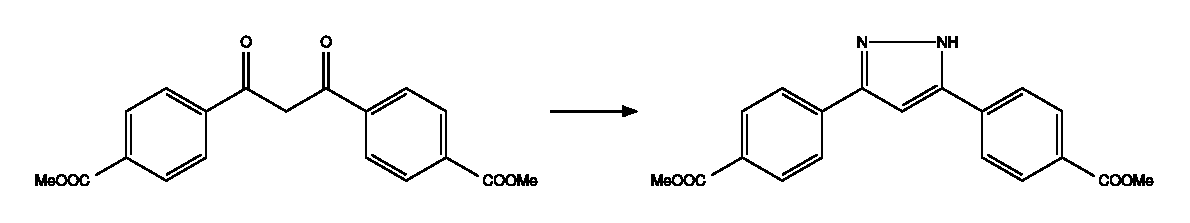
\includegraphics[width=16cm,keepaspectratio]{Structures/pyrazole-formation-appendix.eps}
	\end{figure}
	\begin{table}[h]
		\centering
		\setlength{\tabcolsep}{5pt}     % slight adjustment to fit text width
		\begin{tabular}{cccccccc}
			\toprule
			% \multicolumn{6}{c}{\bf \large Direct addition of hydrazine to DikDiEst}                                                               \\
			% \midrule
			\bf ID & \bf Solvent & \bf Temperature [K] & \bf Reaction time [h] & \bf Hydrazine equivalent & \bf Catalyzer   & \bf Notes & \bf Yield      \\
			\midrule
			01     & EtOH        & 351 (reflux)        & 4                     & 2.5                      & -               & -         & -              \\
			02     & EtOH        & 351 (reflux)        & 17                    & 5                        & \(H_{2}SO_{4}\) & -         & -              \\
			02     & EtOH        & 351 (reflux)        & 17                    & 5                        & TEA             & -         & \(< 5\)        \\
			04     & EtOH        & 351 (reflux)        & 20                    & 10                       & -               & -         & -              \\
			05     & EtOH        & 351 (reflux)        & 17                    & 5                        & \(Et_{4}NOH\)   & -         & -              \\
			06     & DMSO        & 363                 & 10                    & 5                        & -               & -         & -              \\
			07     & DMSO        & 393                 & 24                    & 5                        & -               & -         & -              \\
			08     & DMSO        & 423                 & 24                    & 5                        & TEA             & -         & -              \\
			10     & DMSO        & 423                 & 24                    & 5                        & -               & -         & \(\approx 25\) \\
			11     & THF         & 339                 & 36                    & 5                        & -               & -         & -              \\
			12     & DMF         & 393                 & 17                    & 5                        & -               & -         & \(< 10\)       \\
			\bottomrule
		\end{tabular}
	\end{table}
	\vspace*{\fill}
	\newpage
	\thispagestyle{empty}
	\vspace*{\fill}
	\section{Coniugate addition of hydrazine to UnsDiEst}
	\begin{figure}[h!]
		\centering
		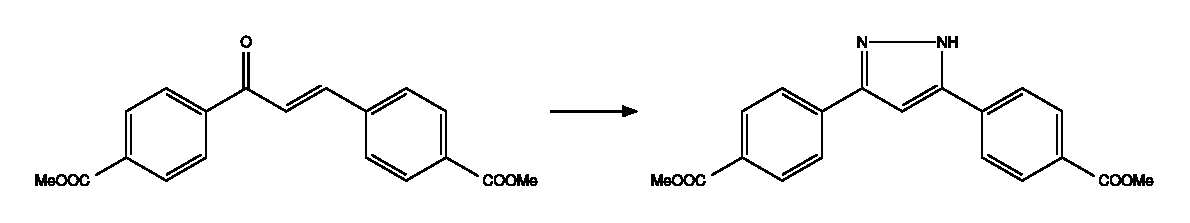
\includegraphics[width=16cm,keepaspectratio]{Structures/pyrazole-formation-appendix2.eps}
	\end{figure}
	\vspace{0.5cm}
	\begin{table}[h]
		\setlength{\tabcolsep}{10pt}     % slight adjustment to fit text width
		\centering
		\begin{tabular}{cccccccc}
			\toprule
			% \multicolumn{6}{c}{\bf \large Coniugate addition of hydrazine to UnsDiEst}                                                            \\
			% \midrule
			\bf ID & \bf Solvent & \bf Temperature [K] & \bf Reaction time [h] & \bf Hydrazine equivalent & \bf Catalyzer & \bf Notes       & \bf Yield \\
			\midrule
			11     & AcOH        & 363                 & 3                     & 3                        & -             & -               & -         \\
			12     & AcOH        & 391 (reflux)        & 17                    & 3                        & -             & -               & -         \\
			12     & MeOH        & 338 (reflux)        & 17                    & 3                        & -             & -               & -         \\
			14     & MeOH        & 338 (reflux)        & 5                     & 3                        & HCl           & -               & -         \\
			15     & MeOH        & 338 (reflux)        & 5                     & 3                        & Pyridine      & -               & -         \\
			16     & MeOH        & RT                  & 17                    & 3                        & -             & -               & -         \\
			17     & EtOH        & RT                  & 5                     & 3                        & -             & -               & -         \\
			18     & AcOH        & 353                 & 0.25                  & -                        & -             & \footnotemark{} & -         \\
			\bottomrule
		\end{tabular}
	\end{table}
	\footnotetext{Microwave 3OO W, starting from idrazone intermediate}.
	\endgroup
	\thispagestyle{empty}
	\vspace*{\fill}

\end{landscape}
\thispagestyle{empty}
\chapter{Diagnostic NMR analysis}
\thispagestyle{empty}
\section{Idrazone intermediate}\label{ap:intermediate}
\begin{figure}[h!]
	\centering
	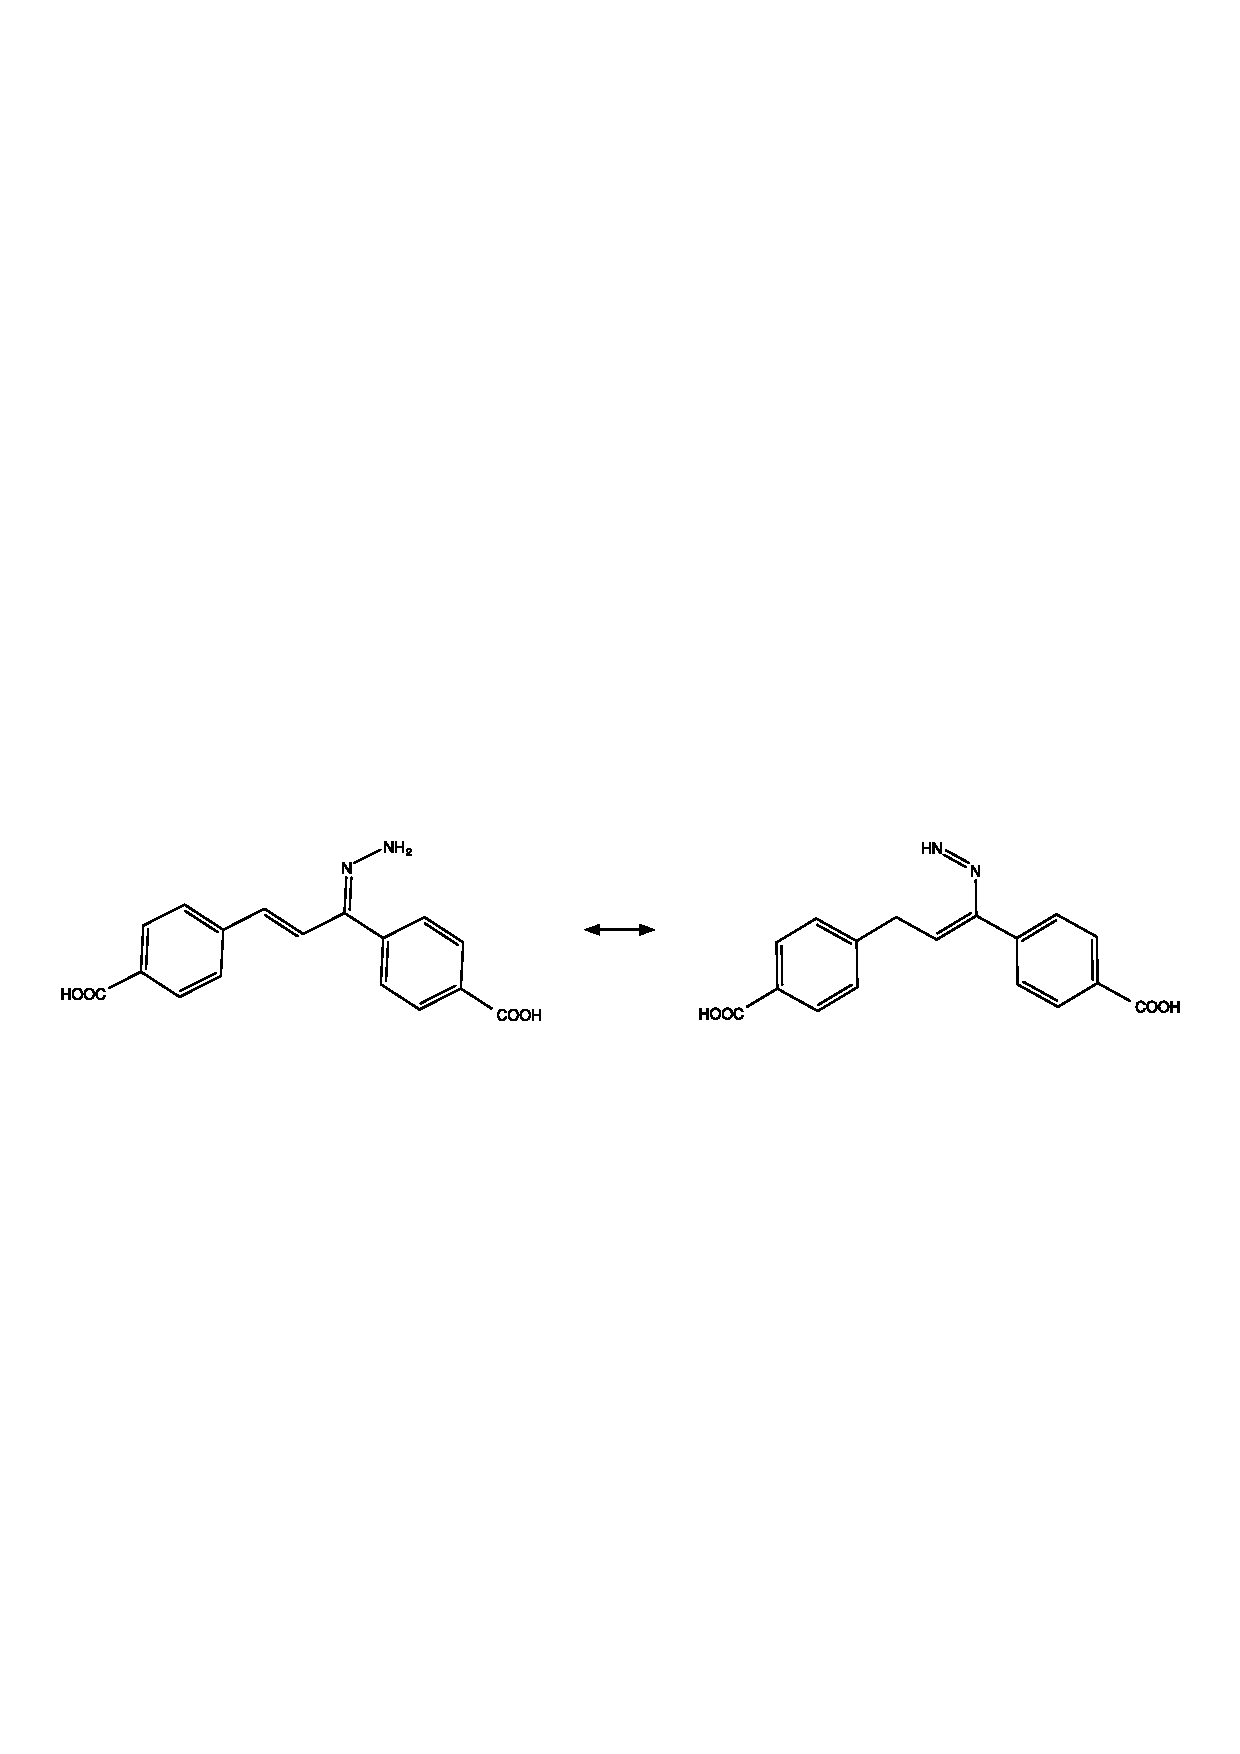
\includegraphics[width=16cm,keepaspectratio]{Spectra/nmr/idrazone.pdf}
	\caption{Idrazone intermediate \NMR*{1,H}(400)[DMSO-d6]}
\end{figure}
\thispagestyle{empty}
\begin{figure}[h!]
	\centering
	\includegraphics[width=16cm,keepaspectratio]{Spectra/nmr/idrazone2.pdf}
	\caption{Idrazone intermediate \NMR*{1,H}(400)[DMSO-d6], zoom on diagonistic peaks}
\end{figure}
\thispagestyle{empty}
\begin{figure}[h!]
	\centering
	\includegraphics[width=16cm,keepaspectratio]{Spectra/nmr/idrazonecosy.pdf}
	\caption{Idrazone intermediate \NMR*{1,H}(400)[DMSO-d6] COSY}
\end{figure}
\thispagestyle{empty}
\begin{figure}[h!]
	\centering
	\includegraphics[width=16cm,keepaspectratio]{Spectra/nmr/idrazonenoesy.pdf}
	\caption{Idrazone intermediate \NMR*{1,H}(400)[DMSO-d6] NOESY}
\end{figure}

\thispagestyle{empty}
\chapter{Complete plotty code}\label{ap:code}

% For completeness below is the program code in its entirety. There are several comments identified by the ``\#' symbol and highlighted in red that make it easier to read and were found to be essential in the writing.
\newline
\lstinputlisting[style=mystyle]{References/PlotCLI.py}
\end{document}

%%% Local Variables:
%%% mode: latex
%%% TeX-master: "../Master"
%%% End:
